%--------------------------------------------------------------------------------------%--------------------------------------------------------------------------------------
%
%  Global settings, dont change it! (excapt additional \usepackage commands)
%  Always use PDFLatex!
%
%--------------------------------------------------------------------------------------%--------------------------------------------------------------------------------------
\documentclass[a4paper, 12pt, oneside, BCOR1cm,toc=chapterentrywithdots]{scrbook}

\usepackage{graphicx}           % use for pdfLatex
\usepackage{makeidx} % f\"{u}r Benutzung des Befehls \printindex
\usepackage[colorlinks=false]{hyperref}
\usepackage{tocbibind}
\usepackage{blindtext}
%\usepackage{subfigure}  %subcaption package is used instead
\usepackage{caption}
\usepackage{subcaption}
\usepackage{acronym}

\usepackage{xcolor}
\usepackage{listings}
\usepackage{adjustbox}

\definecolor{codegreen}{rgb}{0,0.6,0}
\definecolor{codegray}{rgb}{0.5,0.5,0.5}
\definecolor{codepurple}{rgb}{0.58,0,0.82}
\definecolor{backcolour}{rgb}{0.95,0.95,0.92}

\lstset{ 
    language=C++, % choose the language of the code
    basicstyle=\ttfamily\footnotesize,
    keywordstyle=\color{magenta}\bfseries, % style for keywords
    numbers=left, % where to put the line-numbers
    numberstyle=\tiny\color{codegray}, % the size of the fonts that are used for the line-numbers     
		numbersep=5pt,
    backgroundcolor=\color{backcolour},
		commentstyle=\color{codegreen},
    showspaces=false, % show spaces adding particular underscores
    showstringspaces=false, % underline spaces within strings
    showtabs=false, % show tabs within strings adding particular underscores
    %frame=single, % adds a frame around the code
    tabsize=2, % sets default tabsize to 2 spaces
    rulesepcolor=\color{gray},
    rulecolor=\color{black},
    captionpos=b, % sets the caption-position to bottom
    breaklines=true, % sets automatic line breaking
    breakatwhitespace=false, 
}

\definecolor{delim}{RGB}{20,105,176}
\definecolor{numb}{RGB}{106, 109, 32}
\definecolor{string}{rgb}{0.64,0.08,0.08}

\lstdefinelanguage{json}{
    numbers=left,
    numberstyle=\tiny\color{codegray},
		backgroundcolor=\color{backcolour},
    %frame=single,
    rulecolor=\color{black},
    showspaces=false,
    showtabs=false,
    breaklines=true,
    postbreak=\raisebox{0ex}[0ex][0ex]{\ensuremath{\color{gray}\hookrightarrow\space}},
    breakatwhitespace=true,
    basicstyle=\ttfamily\footnotesize,
    upquote=true,
    morestring=[b]",
    stringstyle=\color{string},
    literate=
     *{0}{{{\color{numb}0}}}{1}
      {1}{{{\color{numb}1}}}{1}
      {2}{{{\color{numb}2}}}{1}
      {3}{{{\color{numb}3}}}{1}
      {4}{{{\color{numb}4}}}{1}
      {5}{{{\color{numb}5}}}{1}
      {6}{{{\color{numb}6}}}{1}
      {7}{{{\color{numb}7}}}{1}
      {8}{{{\color{numb}8}}}{1}
      {9}{{{\color{numb}9}}}{1}
      {\{}{{{\color{delim}{\{}}}}{1}
      {\}}{{{\color{delim}{\}}}}}{1}
      {[}{{{\color{delim}{[}}}}{1}
      {]}{{{\color{delim}{]}}}}{1},
}
\hypersetup{%
bookmarksnumbered=true, hyperindex=true,
%
%Im Acrobat Reader Subtitel 1. Ebene anzeigen
bookmarksopen=true, bookmarksopenlevel=1,
%
pdfborder=0 0 0 % Keine Box um die Links!
}

% --------------------------------------------------------------
% Force Tables and List to be added in Table of Content
% --------------------------------------------------------------

\renewcommand*{\tableofcontents}{%
  	\begingroup
  	\tocsection
  	\tocfile{\contentsname}{toc}
  	\endgroup
}
\renewcommand*{\listoffigures}{%
  	\begingroup
  	\tocsection
  	\tocfile{\listfigurename}{lof}
  	\endgroup
}
\renewcommand{\listoftables}{
	\begingroup
	\tocsection
	\tocfile{\listtablename}{lot}
	\endgroup
}
\begin{document}

%--------------------------------------------------------------------------------------%--------------------------------------------------------------------------------------
%
%  Here starts the userspace !
%
%--------------------------------------------------------------------------------------%--------------------------------------------------------------------------------------

%--------titlepage
\begin{titlepage}

{
    \begin{center}
        \raisebox{-1ex}{
\includegraphics[scale=1.5]{TU_Chemnitz_positiv_gruen.pdf}}\\
    \end{center}
    \vspace{0.5cm}
}

\begin{center}

\LARGE{\textbf{Realization of communication with SOME/IP stack over Ethernet}}\\
\vspace{1cm}

\Large{\textbf{Research Internship}}\\ 
\vspace{1cm}

Submitted in Fulfilment of the\\
Requirements for the Academic Degree\\
M.Sc.\\

\vspace{0.5cm}
Dept. of Computer Science\\
Chair of Computer Engineering\\

\end{center}
\vspace{0.6cm}
Submitted by: Sreedhar Hegde\\
Student ID: 671453\\
Submitted On: 12.04.2022\\
\vspace{0.5cm}\\
Supervising tutor: Prof. Dr. W. Hardt \\
\vspace{0.5cm}\\
Company Supervising tutor: M.Eng. Rick Podszuweit

\end{titlepage}

%---------------------------------------------------------
% Abstract
%---------------------------------------------------------
\addchap*{Company Overview}
"`IAV GmbH (Ingenieurgesellschaft Auto und Verkehr), abbreviated to IAV GmbH, is an engineering company in the automotive industry, designing products for powertrain, electronics and vehicle development. Founded in Berlin in 1983 by Prof. Dr. Hermann Appel as a university-affiliated research institute, the company employs over 8,200 members of staff, and supplies automobile manufacturers and suppliers. In addition to development centres in Berlin, Chemnitz and Gifhorn, IAV operates at sites in France, United Kingdom, China, India, Japan, South Korea, Brazil and the United States"'.

The internship work is carried out in the Vehicle Software Solutions Department at Kauffahrtei 25, Chemnitz Location. Vehicle functions increasingly consist of software-based and software-defined systems and account for a large share of the value chain. The Vehicle Software Solutions department is involved in the with the highest series requirements for functional safety and security. The department is a strategic partner for software development, with key competencies in the embedded software development which includes development of software for basic and functional software, the development and integration of systems solutions for serial use and software developement for Automotive Ethernet. The department also owns responsibility for pre-development work and establishment of methodical approaches.

\addchap*{Acknowledgments}
This report is written to fulfill the requirement of the academic degree of M.Sc. Automotive Software Engineering from Faculty of Computer Science, Department of Computer Engineering at the Technical University of Chemnitz. The internship work would not exist without the cooperation between TU Chemnitz and IAV GmbH.

First of all, I would like to express my gratitude to Prof. Dr. Wolfram Hardt for giving me the opportunity to work under his department. Also, I am grateful for his guidance and advice during my studies at TU Chemnitz.

I am grateful to my supervisor Mr. Rick Podszuweit and my manager Mr. Stephan Reichelt, IAV GmbH, for providing me with all facilities, tools and information to complete this work and to achieve the best results during all the phases of the work. Also, I would like to thank them for their guidance without which it would not be possible to successfully complete this internship.

Finally, I would like to express my gratitude to my family and friends for supporting me during my all education phases and encourage me to continue my studies in Germany. 

\addchap*{Abstract}

  

%\textbf{Keywords: Keyword1, Keyword2, Keyword3, ...max 5}

%---------------------------------------------------------
% Table of Contents, List of figures, List of Tables
%---------------------------------------------------------

\tableofcontents
\listoffigures
\listoftables

%---------------------------------------------------------
% List of Abbreviations
%---------------------------------------------------------
\twocolumn
\addchap{List of Abbreviations}
\begin{acronym}[Bash]
 \acro{ADAS}{Advanced Driver Assistance
Systems}
\acro{ARXML}{AUTOSAR XML}
 \acro{API}{Application Program Interface}
 \acro{AUTOSAR}{Automotive Open System
Architecture}
\acro{AVB}{Audio Video Bridging}
\acro{BSW}{Basic Software}
 \acro{CAN}{Controller Area Network}
\acro{COVESA}{Connected Vehicle Systems Alliance}
\acro{DDS}{Data Distribution Service}
 \acro{DoIP}{Diognastic over IP}
 \acro{ECU}{Electronic Control Unit}
\acro{eSOC}{Embedded Service-Oriented Communication}
 \acro{Eth}{Ethernet}
\acro{GUI}{Graphical User Interface}
 \acro{IEEE}{Institute of Electrical and Electronics Engineers}
\acro{IoT}{Internet of Things}
\acro{IP}{Internet Protocol}
\acro{ISO}{International Organization for
Standardization}
\acro{IVN}{In-vehicle Networking}
\acro{JSON}{JavaScript Object Notation}
\acro{LIN}{Local Interconnect Network}
\acro{MAC}{Media Access Control}
 \acro{MOST}{Media Oriented Systems Transport}
  \acro{OEM}{Original Equipment Manufacturer}
 \acro{OS}{Operating Systems}
 \acro{OSI}{Open System Interconnection}
 \acro{PDU}{Protocol Data Unit}
 \acro{PHY}{Physical Layer}
\acro{POSIX}{Portable Operating System Interface}
\acro{RPC}{Remote Procedure Calling}
 \acro{SOA}{Service Oriented Architecture}
 \acro{SOME/IP}{Scalable service-Oriented MiddlewarE over IP}
\acro{SOME/IP-SD}{Scalable service-Oriented MiddlewarE over IP- Service Discovery}
\acro{SWC}{Software Component}
\acro{TCP}{Transmission Control Protocol}
\acro{UDP}{User Datagram Protocol}
\acro{V2X}{Vehicle-to-Anything communication}
\end{acronym}

\onecolumn
%---------------------------------------------------------
% Here starts the real work
%---------------------------------------------------------

\chapter{Introduction}
% just insert your text here

Communication is essential in modern vehicles to establish a link between the ECUs in the network. In addition, as the number of ECUs and high-performance controllers grows, so does the need for more bandwidth than traditional in-vehicle networks such as CAN, Flexray, and MOST can provide. With the introduction of Ethernet into the automotive domain, bandwidths of up to 1 Gb/s can now be achieved within the vehicle network. The use of Ethernet benefits systems such as ADAS and infotainment significantly. However, in order to transmit and receive data at a significantly high data rate, a robust communication control mechanism is required. The use of Ethernet benefits systems such as ADAS and infotainment substantially. However, in order to transmit and receive data at a remarkably high data rate, a robust communication control mechanism is required. With the growing interest in POSIX-based systems in the automotive domain, service oriented architecture (SOA) plays an important role in meeting the needs of technology-driven applications. The core of SOA is remote procedure calling (RPC) and the Client-Server mechanism. To realize these concepts, there is a need for a middleware that is specifically designed to run automotive applications smoothly. To accomplish this, SOME/IP middleware was introduced in the automotive context. As more applications migrate to Adaptive AUTOSAR, SOME/IP is well suited to serve as a communication control protocol alongside existing communication technologies.

This report conducts a thorough examination of the SOME/IP technology. In Chapter 2, the details of the current systems and the most recent technology are explained. The open source library vsomeip provided by GENIVI is used to understand the functioning of SOME/IP technology. A demonstrator is set up, consisting of target hardware running on various underlying architectures such as x64, armv7, and armv8. The devices are linked together on a network via Ethernet. The functionality is achieved by running applications based on the vsomeip stack on these hardware devices. In Chapter 3, these concepts and their implementation are explained in detail. The fourth chapter focuses on the implementation's outcomes.The fourth chapter focuses on the outcomes of the implementation. As a reference document, a troubleshooting guide containing the most commonly encountered issues and faults when using SOME/IP technology has also been documented. Chapter 5 provides a conclusion to this report as well as the future scope of the work.  % Load Data from File intro.tex

\chapter{Literature Survey}
\section{Communication technologies in Automotive Domain}
More than 100 ECUs connect via in-vehicle buses in modern vehicles\cite{b1.0}. As a result, there is a greater need than ever for a dependable communication network with high bandwidth. In order to meet these requirements, BMW implemented Ethernet for the first time in vehicles in 2013. At the same time, it is important to note that the incorporation of Ethernet as an in-vehicle networking system does not imply that traditional communication networks such as CAN, LIN, and MOST are rendered obsolete. Because these networks are robust, inexpensive, time-tested, and provide necessary performance for many applications, Automotive Ethernet will not completely replace them, but will supplement them to provide even more cost, performance, and feature benefits. Table \ref{tab:Comparison_Automotive_Networks} shows the important characteristics of automotive networks in comparison with the Ethernet.
\begin{center}
\begin{tabular}{|c|c|c|c|c|c|c}
\hline
\textbf{Property} & \textbf{Ethernet} & \textbf{CAN} & \textbf{FlexRay} & \textbf{MOST} & \textbf{LIN}\\
\hline
Bandwidth(Mb/s) & \textgreater 100 & 1 & 20 & 150 & 0.02\\
\hline
Nodes & Scalable & 30 & 22 & 64 & 16\\
\hline
Network Length & 15m per link & 40m & 24m & 1280m & 40m\\
\hline
%Media Access Control & Full-duplex contention less & Non-destructive arbitration & Time-triggered & Time-triggered & Time-triggered\\
Topologies & Star, Tree & Bus& Bus,start & Ring,Star & Bus\\
\hline
Cost & High& Low& Low& High& Very low\\
\hline
Cabling & UTP & UTP & UTP & Optical,UTP & 1-wire\\

\hline
\end{tabular}
\captionof{table}{Comparison of important characteristics of automotive networks \cite[p.202]{b1}}
\label{tab:Comparison_Automotive_Networks}
\end{center}

\section{Ethernet in the Automotive Domain}
\label{sec:EthernetInTheAutomotiveDomain}
In the year 1980, consumer-oriented Ethernet was introduced. However, Ethernet use in the automotive domain did not begin until 2013. This was due to EMC emissions levels being higher than those required for vehicle use. The introduction of BroadR-Reach twisted pair cables meant that the stringent EMC performance regulations were met and that the cables could finally be used in the automotive domain. Initially, Ethernet 100BASE-TX was used for OBD and updating the ECUs' flash memories\cite{b1.0.1_AE_History}. It has also been used for applications relating to infotainment and camera systems over the years. With an increasing number of sensors in a vehicle, data acquisition and high-speed communication become essential. In the current scenario, Automotive Ethernet appears to be the most viable solution for meeting these requirements. Also, Automotive Ethernet is said to be the next-generation in-vehicle networking systems when connecting application domains, transporting different kinds of data (control data, streaming, etc.)\cite{b1.0.1_AE_History}.  

\section{Ethernet as backbone in vehicles}
Traditionally, CAN, LIN, FlexRay, and MOST are used as in-vehicle communication technologies\cite{b1.0_EthBackbone}. Although Ethernet is a relatively new to the automotive domain, it offers several desirable properties such as high bandwidth, interoperability, robustness, low cost and seamless integration with the TCP/IP stack\cite{b1.0_EthBackbone}. Because it is a peer-to-peer network with full duplex communication, each ECU can communicate with one another at 100 Mb/s bandwidth. However, in order to meet the delay requirements, complementary technologies such as AVB for in-vehicle communication are required.   

\begin{figure}[!htb]
	\centering
		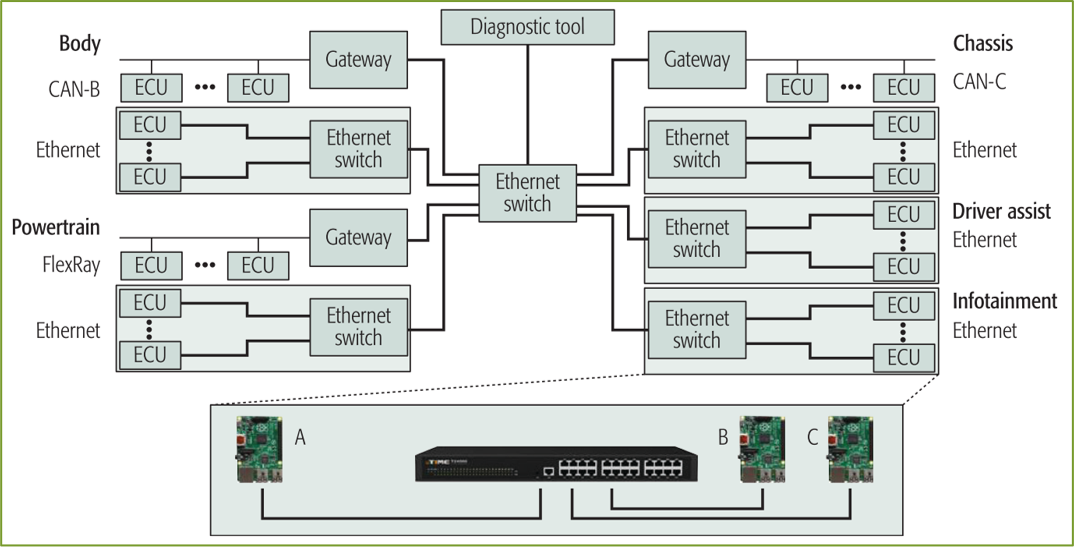
\includegraphics[width=1\textwidth]{images/Switched_Ethernet_backbone.png}
	\caption{Ethernet as a backbone for in-vehicle communication\cite{b1.0_EthBackbone}}
	\label{fig:Switched_Ethernet_backbone}
\end{figure}

\par Figure \ref{fig:Switched_Ethernet_backbone} is an example of an in-vehicle network with Ethernet as a backbone. Low-speed networks such as CAN, LIN, and Flexray are connected to Ethernet via a switch using gateways\cite{b1.0_EthBackbone}. This facilitates the establishment of a link between ECUs that are integrated with Ethernet as the native protocol and have higher bandwidth requirements for their applications, allowing message sharing across domains. With the introduction of IoT in the automotive industry, a switched Ethernet network serves as the foundation technology for implementing V2X communication.


\section{Service Oriented Architecture}
Automotive Ethernet has resulted in a paradigm shift in the development of automotive systems. Because scalability is one of the primary advantages of using Automotive Ethernet, newer protocols and technologies that provide smooth, flexible, and scalable software solutions are required. SOA is one of the tried-and-true web services technologies that can be applied in the automotive context to support the growing complexity of automotive software. Given the resource limitations of ECUs, the SOA protocols designed for high level machines and servers cannot be directly used for the automotive software. In order to bridge the gap and reuse the concepts of the existing SOA model, new protocols are needed to be developed. AUTOSAR provides a standardized specifications for a protocols such as SOME/IP and DDS which works by incorporating the concepts of the SOA model. The details of these technologies are discussed in the following section.   

\section{Middleware in the automotive domain}
The increasing complexity in the automotive applications means there is a need for standardized middleware that can provide common services and common interfaces to the application software components\cite{b_TrendsInACS}. Middleware is a software layer that connects and manages application components running on distributed hosts\cite{b_middleware}. In practice, a middleware is composed of a collection of existing communication protocols and carmarker-specific layers\cite{b_TrendsInACS}. In the context of communication control, the middleware's role is to provide a layer of abstraction between the application software and the network.\cite{b1.4}. AUTOSAR has standardized specifications for middleware such as SOME/IP and DDS. Apart from this several other middleware based on CAN protocol such as eSOC\cite{b_TrendsInACS} are available for use in the automotive context. 

\subsection{SOME/IP}
``Scalable service Oriented MiddlewarE over IP" abbreviated SOME/IP represents a middleware that was created for automotive use cases \cite{b1.1}. The compatibility with AUTOSAR was a necessity regarding SOME/IP at least on wire-format level \cite{b1.1}. SOME/IP communication is an exchange of messages between different devices like ECUs over IP \cite{b1.1}. The SOME/IP protocol aims to define a uniform middleware for IP-based communication within vehicles. Table \ref{ISO_OSI_Model} represents the organization of the SOME/IP middleware in the ISO/OSI model.
\par  

\begin{center}
		\begin{tabular}{|c|c|}
		\hline
			7 & \\
			6 & SOME/IP \\
			5 & \\
		\hline
			4 & TCP/UDP \\
		\hline
			3 & IPv4/IPv6 \\
		\hline
		2 & Eth.MAC/IEEE DLL \\
		\hline
		1 & Ethernet PHY \\
		\hline			
		\end{tabular}
	\captionof{table}{Simplified ISO/OSI model of Automotive Ethernet stack for communication control}
	\label{ISO_OSI_Model}
\end{center}

The protocol builds on top of an existing TCP/UDP stack, adding another level of abstraction for application communication by enabling locality transparency. This property denotes the fact that an application has no knowledge of which network node provides the desired function or information. If the desired function or information is available on the same ECU, a local connection is established between the software components \cite{b1.4}. When the information, on the other hand, is on another node on the same network, the middleware performs the necessary network communication and provides the data to the application.

\begin{figure}[!htb]
	\centering
		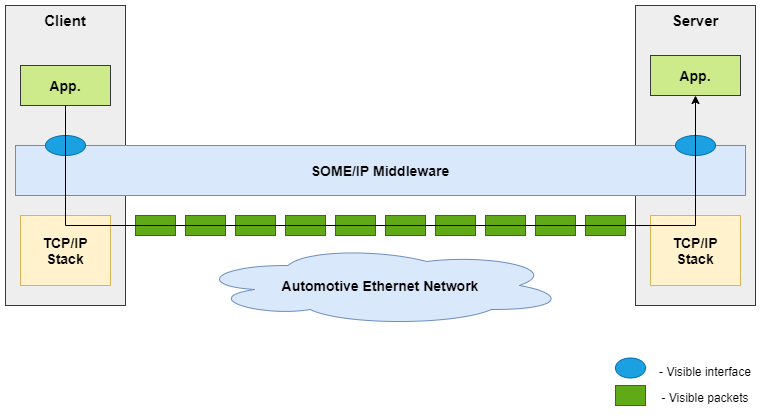
\includegraphics[width=1\textwidth]{images/SOMEIP_Middleware.png}
	\caption{SOA representation with SOME/IP middleware}
	\label{fig:SOMEIP_Middleware}
\end{figure}

Figure \ref{fig:SOMEIP_Middleware} depicts a high-level overview of the SOME/IP transformer. It is based on the client-server mechanism used in service-oriented architecture. This enables a variety of methods for sending and requesting data between the client and server via RPCs and Publish-Subscribe models. The following section describes the specifics of these communication methods.

\subsubsection{Communication methods}
\label{sec:CommunicationMethods}

\begin{figure}[!htb]
	%\centering
		\begin{subfigure}[b]{.5\textwidth}
		%	\centering
				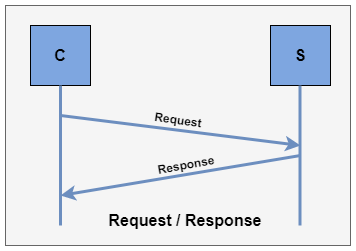
\includegraphics[width=\textwidth]{images/Request-response.png}
				\caption{``Request-Response"'-RPC: method call with response message}
				\label{fig:Request-response}
		\end{subfigure}		
		\begin{subfigure}[b]{.5\textwidth}
		%	\centering
			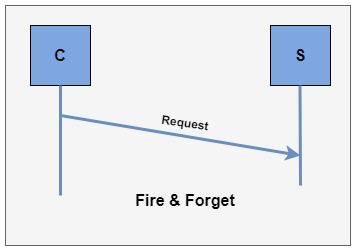
\includegraphics[width=\textwidth]{images/fire-forget.png}
			\caption{``Fire \& Forget"'- RPC: Method call without a response}
			\label{fig:fire-forget}
		\end{subfigure}
		\begin{subfigure}[b]{.5\textwidth}
			%\centering
				 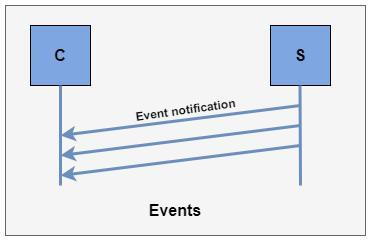
\includegraphics[width=\textwidth]{images/Events.png}
				\caption{``Publish-Subscribe - Events"': Event notifications}
				%\caption{fig 1}
				\label{fig:Events}
		\end{subfigure}
		\begin{subfigure}[b]{.5\textwidth}
			%\centering
				 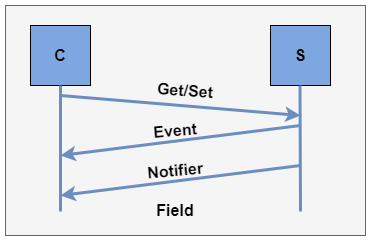
\includegraphics[width=\textwidth]{images/Field.png}
				\caption{``Fields"': Set or read out the data fields of
another service.}
				%\caption{fig 1}
				\label{fig:Field}
		\end{subfigure}
	\caption{SOME/IP communication types between clients and servers}
\end{figure}










\chapter{Implementation}
To demonstrate the use of the SOME/IP technology, several devices (target controllers) are connected within a network and communication is established between them using Ethernet. In this chapter, the requirements to visualize the technology are explained and also the procedure to setup the demonstrator is discussed in detail. 

\section{Concept}
Figure \ref{fig:Visual_representation_of_hardware_setup} depicts the physically interconnected hardware in the hardware setup. The prototype is made up of a computer running a virtual machine\cite{b_hyperv}, a Raspberry Pi 3b+ \cite{b_raspi3b}, and an Odroid XU4\cite{b_odroidxu4}. A routing device connects the devices to the same network via ethernet cables. Each of the target hardware have different target architecture. The overall objective is to showcase the technology by running it simultaneously on several architectures. These devices represent the target ECUs within a vehicle that are responsible for performing specific functions based on information exchanged with SOME/IP as the underlying technology.

\begin{figure}[!htb]
	\centering
		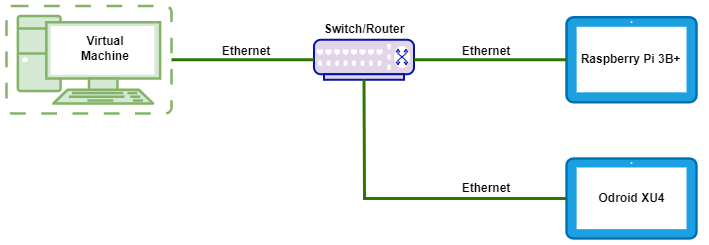
\includegraphics[width=1\textwidth]{images/Visual_representation_of_hardware_setup.png}
	\caption{Visual representation of the hardware setup}
	\label{fig:Visual_representation_of_hardware_setup}
\end{figure}
\par In order to implement the applications to visualise the usage of technologies several open source stacks such as scapy-someip \cite{scapy_someip}, the GENIVI vsomeip stack  \cite{b_genivi_vsomeip}, Rust based SOME/IP implementation \cite{rust_someip} were investigated. COVESA's (formerly known as GENIVI's) vsomeip stack appeared to be the most appropriate of the currently available implementations for this activity as it is based on POSIX and uses C++ programming language for the implementation. With the trend toward using Adaptive AUTOSAR\cite{b_adaptive_platform} in application software development, it provides as a major motivation to realize the concepts in a POSIX-based environment. 
\par Figure \ref{fig:SOMEIP_concept} shows the software stack and the endpoints in each of the hardware setup. A virtual machine is setup in the windows PC to emulate a Linux based environment. The devices Raspberry Pi 3b+ and Odroid XU4 are also setup with a Linux operating system. Further, these devices are installed with certain software and libraries that are required to setup the environment to demonstrate the technology. The GENIVI vsomeip stack is used to build the target applications on each of the devices. There can be multiple SOME/IP applications running on these devices. However, only one routing manager is allowed per device. The role of the routing manager is to help in routing the incoming and outgoing messages to the appropriate destinations. With access to the TCP/UDP endpoints, the devices can communicate with each other via Ethernet as shown in the figure \ref{fig:SOMEIP_concept}. 
 
\begin{figure}[!htb]
	\centering
		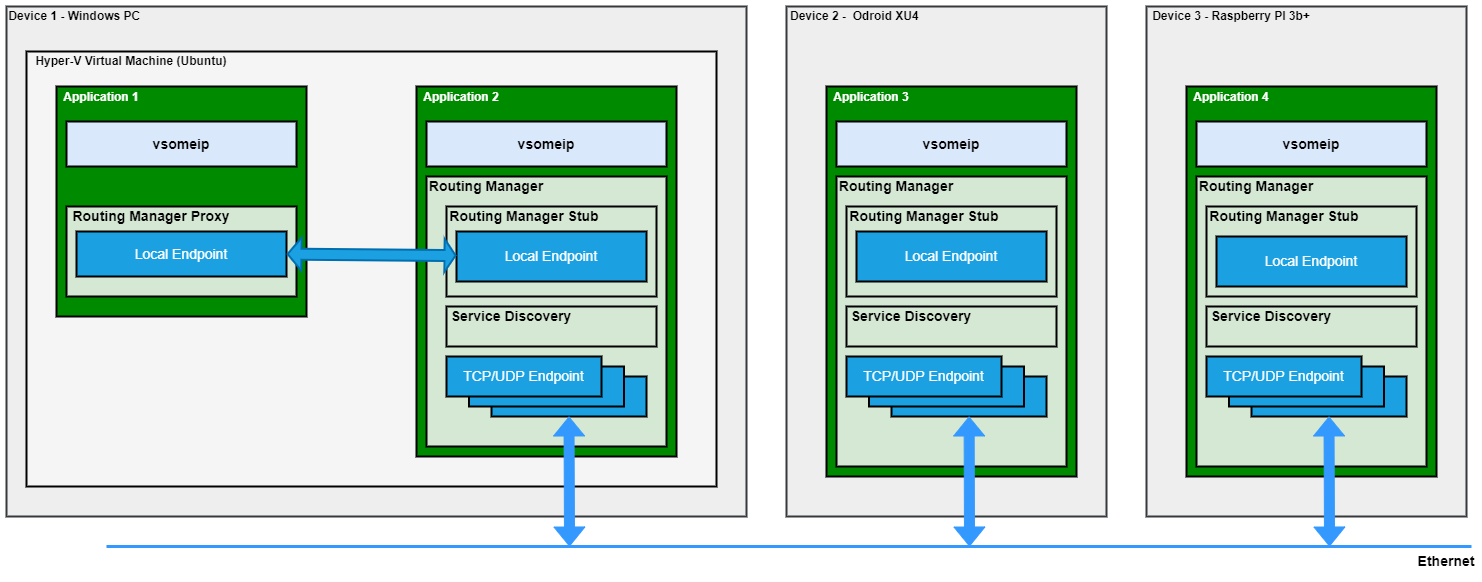
\includegraphics[width=1\textwidth]{images/SOMEIP_concept.png}
	\caption{SOME/IP concept}
	\label{fig:SOMEIP_concept}
\end{figure}

\section{Target Hardware}
\subsection{Virtual Machine}
The Hyper-V virtualization platform from Microsoft is used to host POSIX-based environments on a Windows PC. Alternatively, other virtualization platforms can also be used for the same purpose. Based on the license constraints and availability, Hyper-V has been chosen for this project.  An i386 (x86) architecture compatible OS is required to be hosted based on the concept design. For this activity, the open source Linux OS Ubuntu 20.04 LTS has been chosen for hosting on this platform. In this virtual environment, the necessary software for demonstrating the use of the technology is then installed. The physical Ethernet port on the PC is mapped to the virtual machine in order for it to communicate with the other target hardware.

\subsection{Raspiberry Pi 3b+}
The Raspberry Pi 3b+ is a single-board computer (SBC) with an ARM cortexA53 processor that is commonly used for home automation projects and prototyping. It has 1GB LPDDR2 SDRAM as well as built-in Gigabit Ethernet support. It also supports the installation of a POSIX-based environment on the board, making it appropriate for this project. For demonstration purposes, a lightweight 64-bit DietPi OS along with relevant library packages are setup on this device.

\subsection{Odroid XU4}
Odroid XU4 is an energy-efficient powerful ARM-based computing hardware that can run a variety of Linux operating systems, including Ubuntu 18.04 and Android 7.1 Nougat. It has 2GB of LPDDR3 RAM as well as Gigabit Ethernet interface support, which is required to implement SOME/IP communication concepts. As a result, this makes for good prototyping hardware because the target library packages can be configured to run the target applications on this device.

\section{Software}
\subsection{Target Libraries}
SOME/IP application development necessitates the use of several prerequisite stacks and libraries. This section contains a list of the required libraries as well as a brief overview of the libraries. All of the libraries used in this project are open source and can be used commercially. These libraries must be built for each target hardware in order for the applications to run on the devices. In this project, the target libraries are cross-compiled on the virtual machine, and the binaries are then copied to each of the devices. The following section goes over the specifics of cross-compilation.

\subsubsection{GENIVI vsomeip stack}
\subsubsection{CommonAPI}
CommonAPI C++ is a standardized C++ API specification for the development of distributed applications which communicate via a middleware for interprocess communication\cite{b_commonapi}. The main intention is to make the C++ interface for applications independent from the underlying IPC stack\cite{b_commonapi}.


\subsubsection{Boost}


\subsection{Tools}
\subsubsection{Qt Creator}
Qt Creator is a cross-platform integrated development environment (IDE) built for the maximum developer experience\cite{b_QtCreator}. Qt Creator runs on Windows, Linux, and macOS desktop operating systems, and allows developers to create applications across desktop, mobile, and embedded platforms\cite{b_QtCreator}. The GUI for the SOME/IP-based applications is built for demonstration purposes using the open source version v5.0 of the Qt creator.

\subsubsection{CMake}
CMake is a tool to manage building of source code\cite{b_CMake}. CMake is widely used for the C and C++ programming languages, but it can also be used to generate source code for other languages\cite{b_CMake}. Originally intended as a generator for various dialects of Makefile, CMake now generates project files for modern buildsystems such as Ninja as well as project files for IDEs such as Visual Studio and Xcode\cite{b_CMake}. CMake is used as the build system in this project for compilation as well as cross-compilation of library packages and SOME/IP applications for different target hardware.

\subsubsection{PuTTY}
PuTTY is an SSH and telnet client, developed originally by Simon Tatham for the Windows platform\cite{b_putty}. PuTTY is open source software that is available with source code and is developed and supported by a group of volunteers\cite{b_putty}. This tool is required to run the terminals for Raspberry Pi3b+ and Odroid XU4 remotely on the host machine. This enables to smoothly switch between the target devices when running the applications on the target hardware respectively.

\section{Cross-compilation}
Every development board is embedded with a specific amount of RAM, storage capacity, input and output peripherals and other hardware components. Hosting the target environment on multiple boards can be complicated and time consuming. Furthermore, building target libraries on these boards can take a long time and may fail in some cases. To address these issues, it is worthwhile to setup a generic build environment on a single platform and build the projects for different targets accordingly. This process is called as cross-compilation. In this section, the process to setup a cross-compilation environment on the Linux platform is illustrated and along with it, the procedure to cross-compile boost libraries for Raspberry Pi and Odroid XU4 target platforms is demonstrated respectively.

\subsection{Installing cross compilers on the host machine}
In this section, the basic requirements to setup a cross-compilation tool-chain is described. Also, based on the requirements for the demonstration of the SOME/IP technology, build process for libraries such as Boost, CommonAPI, vsomeip and other relevant libraries are described in detail. 
\par In order to cross-compile, appropriate tool-chain packages has to be first setup in the host environment. The commands from the following listings are required to be run in a terminal window in the Linux machine. Please note that an active internet connection is required to download the packages from the server. 

\begin{lstlisting}[language=bash, caption={Command to install packages for ARM 32-bit (armv7) tool-chain}]
  user@machine:~$ sudo apt-get install gcc-arm-linux-gnueabihf
	g++-arm-linux-gnueabihf
\end{lstlisting}

\begin{lstlisting}[language=bash, caption={Command to install packages for ARM 64-bit(armv8) tool-chain}]
  user@machine:~$ sudo apt-get install gcc-aarch64-linux-gnu
	g++-aarch64-linux-gnu
\end{lstlisting}

\begin{lstlisting}[language=bash, caption={Command to install other required packages}]
  user@machine:~$ sudo apt-get install build-essential
	manpages-dev openjdk-8-jdk libssl-dev wireshark 
	g++-aarch64-linux-gnu
\end{lstlisting} 

\section{Demo Application}
In this section, a demo application built with Qt Creator is shown to demonstrate the technology. Two separate applications are created, one for the server ECU and one for the client ECU. These user interface-based applications are used to demonstrate intra-ECU and inter-ECU communication. However, when inter-ECU communication is required, the UI-based application is only run on the virtual machine. The SOME/IP applications are run without the UI on the other target hardware. In the case of inter-ECU communication, for example, when the server application is run on the virtual machine, it is represented by a UI-based application, whereas the client application is run on one of the target hardware without a graphical interface. Each SOME/IP-based communication method is represented on both the client and server applications, with detailed information displayed in a terminal window. The responses received by the client are displayed on the terminal window, which also contains detailed information about the messages sent and received. The specifics of the implementations are covered in the following sections.

\subsection{vsomeip application}
To create a vsomeip application, the libraries described in the preceding sections must be available. To realize the SOME/IP communication types, an application must be written with information containing details such as the name of the application, the services offered, and the services to be requested. A registry handler function must be used to register the services and service instances in a registry. In addition, the application's requested services must be stored in the availability handler registry using the availability handler functions. The vsomeip stack provides APIs for creating a vsomeip application and registering services in the appropriate registry. The code example in the listing \ref{code:init_application} shows a snippet of code from the server application related to the creation of an application and storing information about offered and requested services in the registry handlers. The RPM service denotes the method to create a service that offers request-response type of service. To offer services which supports event notifications, the events have to be inserted in an event group. This is demonstrated using the indicator service. To request a service offered by other vsomeip applications, a service request has to be invoked that includes the service information details. 

\begin{lstlisting}[caption={vsomeip application initial configurations}, label=code:init_application]
#include <vsomeip/vsomeip.hpp>

const char ApplicationName[] = "vsomeip_server";

int main()
{
		//Create a vsomeip application
    app = vsomeip::runtime::get()->create_application(ApplicationName);
		
    bool Is_init_Successful = app->init();
		
    if(Is_init_Successful)
    {
        /*  RPM Service registration
				Macros : RPM_SERVICE_ID 0x2000, RPM_INSTANCE_ID 0x2100, RPM_METHOD_ID 0x2200  */
				//message handler registration. Callback function name: on_message
        app->register_message_handler(RPM_SERVICE_ID, RPM_INSTANCE_ID, RPM_METHOD_ID, on_message);
				//Offer the service to the clients
        app->offer_service(RPM_SERVICE_ID, RPM_INSTANCE_ID);

        /*Indicator service registration
				Macros : INDICATOR_SERVICE_ID 0x2500, INDICATOR_INSTANCE_ID 0x2510, INDICATOR_METHOD_ID 0x2520,
				INDICATOR_EVENTGROUP_ID 0x4400, INDICATOR_EVENT_ID 0x4300  */
        app->register_message_handler(INDICATOR_SERVICE_ID, INDICATOR_INSTANCE_ID, INDICATOR_METHOD_ID, on_message);
        app->offer_service(INDICATOR_SERVICE_ID, INDICATOR_INSTANCE_ID);
        its_groups.insert(INDICATOR_EVENTGROUP_ID);
        app->offer_event(INDICATOR_SERVICE_ID, INDICATOR_INSTANCE_ID, INDICATOR_EVENT_ID, its_groups, true);

        /*Temperature service registration 
				Macros : TEMP_SERVICE_ID 0x2500; TEMP_INSTANCE_ID 0x2510; TEMP_METHOD_ID 0x2520 */
        app->register_message_handler(TEMP_SERVICE_ID, TEMP_INSTANCE_ID, TEMP_METHOD_ID, on_message);
				//Availability handler registration. Callback function name: on_availability
        app->register_availability_handler(TEMP_SERVICE_ID, TEMP_INSTANCE_ID, on_availability);
				//Request temperature service from other server/client
				app->request_service(TEMP_SERVICE_ID, TEMP_INSTANCE_ID);
				
				//Start the application
        app->start();
    }
    else
    {
				//Error message output if application is unable to start
        std::cerr << "Error Code: VS001: Failed to start application: " <<  ApplicationName  << " due to unsuccessful initialization " << std::endl;
    }
}
\end{lstlisting}

The callback function on\_message is demonstrated in listing \ref{code:register_message_callback}. A generic callback function can be used to implement all of the services that are offered and requested, or multiple callback functions can be implemented based on the intended functionality upon the reception of a message from a specific service. In this example listing, a generic callback function is implemented, and the corresponding function call is invoked to provide the intended functionality based on the service ID extracted from the response message header.

\begin{lstlisting}[caption={vsomeip message handler callback}, label=code:register_message_callback]
void on_message(const std::shared_ptr<vsomeip::message> &_RespMsg)
{
	//Get the service ID of the response message
  int ResponseServiceID = (int)_RespMsg->get_service();

	switch(ResponseServiceID)
	{
		//Invoke function related to rpm service
		case RPM_SERVICE_ID: on_rpm_service_Msg(_RespMsg); break;
		//Invoke function related to speed service
		case SPEED_SERVICE_ID: on_speed_service_Msg(_RespMsg); break;
		//Invoke function related to temperature service ID
		case TEMP_SERVICE_ID: on_temp_service_Msg(_RespMsg); break;
		//Invoke function related to fuel service ID
		case FUEL_SERVICE_ID: on_temp_service_Msg(_RespMsg); break;
		//Invoke function related to fuel service ID
		case INDICATOR_SERVICE_ID: on_indicator_service_Msg(_RespMsg); break;
		case default: break;
	}
}
\end{lstlisting}

The listing \ref{code:received_message_processing} shows how to process a received message for RPM service. Once the message has been received, the payload length, sender, message type, and other information can be extracted from the message header. Furthermore, the received data can be processed in order to compute and retrieve the RPM data that is available on the server side. The header information for a response message can be created and sent back to the client based on the type of message received. Data shall not be sent back to the client in the event of a fire and forget communication type. Similarly, messages for other services are processed, and responses are returned as appropriate.

\begin{lstlisting}[caption={Example of received message processing}, label=code:received_message_processing]
on_rpm_service_Msg(const std::shared_ptr<vsomeip::message> &_RespMsg)
{
	//extract the payload from the received response
  std::shared_ptr<vsomeip::payload> its_payload = _RespMsg->get_payload();
	//Get the length of the payload
  vsomeip::length_t payload_len = its_payload->get_length();

  int ResponseMessageType =(int)_response->get_message_type();

  int ResponseServiceID = (int)_response->get_service();

  std::stringstream RecievedResponse;

  //Check if recieve response is related to RPM service
  if((RPM_SERVICE_ID == ResponseServiceID) && (0x00 == ResponseMessageType))
  {
      for (vsomeip::length_t i=0; i < payload_len; i++)
      {
          RecievedResponse << std::setw(2) << std::setfill('0') << std::hex
          << (int)*(its_payload->get_data()+i) << " ";
      }
      //Send the current RPM data from the server
      (void)SendRpmData(_response);
  }
	else
	{
		//Place holder for other response message types
	}
}
\end{lstlisting}

The availability handler callback function is shown in listing \ref{code:availability_handler_callback}. This function is called during the application's initialization phase and remains active throughout. Once the service becomes unavailable, the availability stated also is inverted accordingly. Based on the information stored in the service registry, the vsomeip stack determines whether a service and its instances are available. The end user can be notified if a specific service is available for consumption using the information. In addition, depending on the availability, internal back-end computations related to the service can be started in order to generate the necessary data. Several utility functions are implemented in this demonstration to invoke and compute the required information once a service and its instance are available. Listing \ref{code:availability_handler_utility} is a snippet of an RPM service implementation. When the RPM service becomes available, a thread associated with the RPM service is notified in order to compute the necessary data.
 
\begin{lstlisting}[caption={vsomeip availability handler callback function}, label=code:availability_handler_callback]
void on_availability(vsomeip::service_t _service, vsomeip::instance_t _instance, bool _is_available)
{
    bool IsServiceAvailable_b = util_IsServiceAvailable(_service, _is_available);

    std::cout << "CLIENT-> ["<< ApplicationName << "]" <<": Service ["
            << std::setw(4) << std::setfill('0') << std::hex << _service << "." << _instance
            << "] is "
            << (IsServiceAvailable_b ? "available." : "unavailable. [Error Code: VS003]")
            << std::endl;
}
\end{lstlisting}

\begin{lstlisting}[caption={availability handler utility function}, label=code:availability_handler_utility]
bool util_IsServiceAvailable(const vsomeip::service_t _service, const bool _is_available)
{
    bool IsServiceAvailable_b = false;
    switch(_service)
    {
			case RPM_SERVICE_ID :
        if(_is_available)
        {
            IsServiceAvailable_b = true;
            isRPMservice_avalaible_ = true;
						//Notify the thread related to RPM service once the service ID is available
            (void)RPMRequestThreadNotify();
        }
        break;
    }
    return IsServiceAvailable_b;
}
\end{lstlisting}

\subsection{Server Application}
The server user interface is depicted in Figure \ref{fig:serverUI}. Several different types of information are sent and received between the server and the client for demonstration purposes. The server sends the RPM, Speed, Fuel, and Indicator information to the client. The data for RPM, Speed, and Fuel can all be changed by using the vertical scroll bars. The progress bars represent the information that is dynamically updated. The Request-Response communication type is represented by the RPM information. It means that whenever the client makes a request, the server sends the most up-to-date RPM information to the client. Similarly, the Speed and Fuel information represent field-based event notifications from the server to the client. The information for the left and right indicators can be changed by using the respective buttons on the user interface. Whenever the value is updated, the data is sent out immediately with message type information set to "`MT\_NOTIFICATION"'. The information is sent as event notifications from the server sent to the client. A notification message with service identifier, instance identifier, the client identifier, message type, payload and other details is packed and triggered from the server. The TEMP variable indicates the ambient temperature. The data is sent as a request message from the client to the server, with no expectation of a response message from the server (fire \& forget communication type). The temperature data is stored in the server application and can be used for further processing.

\begin{figure}[!htb]
	\centering
		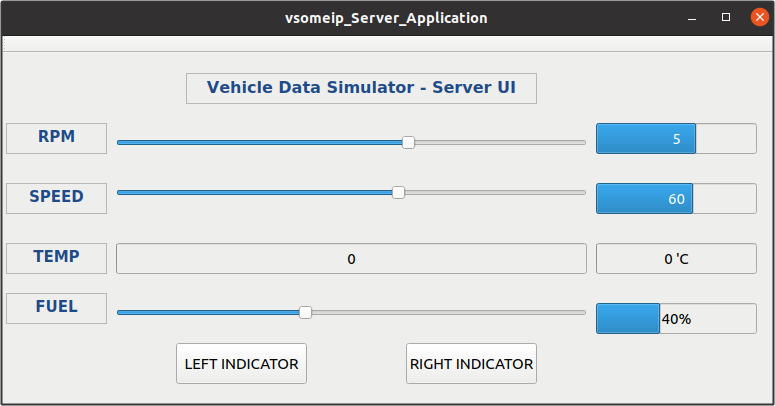
\includegraphics[width=1\textwidth]{images/serverUI.png}
	\caption{Qt based Server application GUI}
	\label{fig:serverUI}
\end{figure}

\subsection{Client Application}
The client user interface is depicted in Figure \ref{fig:clientUI}. Similar to the server user interface, the client user interface consists of graphical elements that represent the information related to RPM, speed, temperature and fuel data. The information on the user interface is dynamically updated as and when the data is recieved from other vsomeip applications. However, the data for RPM is received only when the "`Request RPM"' button is pressed indicating a request for information being triggered to the server. The message type information is set as "`MT\_REQUEST"' indicating a request is placed to the server application. The server application then provides a response with the response message type set to "`MT\_RESPONSE"'.  Also, the ambient temperature value is set by the client and the data is sent to the server whenever the "`Send Current Temp"' button is pressed on the user interface. This information represents the fire \& forget communication type where the data is pushed to the server by the client without requesting any acknowledgment from the server. The receiver application gets this message with type information as "`MT\_REQUEST\_NO\_RETURN"' indicating no further response back to the sender is required.

\begin{figure}[!htb] 

	\centering
		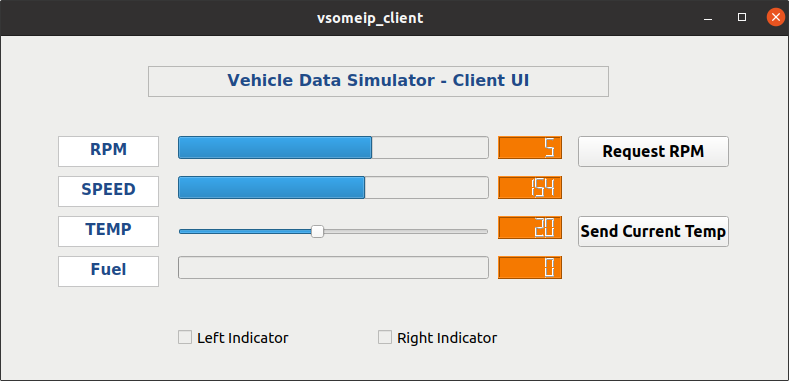
\includegraphics[width=1\textwidth]{images/clientUI.png}
	\caption{Qt based Client application GUI}
	\label{fig:clientUI}
\end{figure}

\subsection{Comunication establishment between devices}
Configuration


\chapter{Results}
Based on the implementation of the SOME/IP technology, the applications are run on the target hardware to realize the outcome. In this chapter, the results of several scenarios of the technology are presented and a brief overview of the troubleshooting guide is discussed.

\subsection{Server Application Output}
\begin{figure}[!htb]
	\centering
		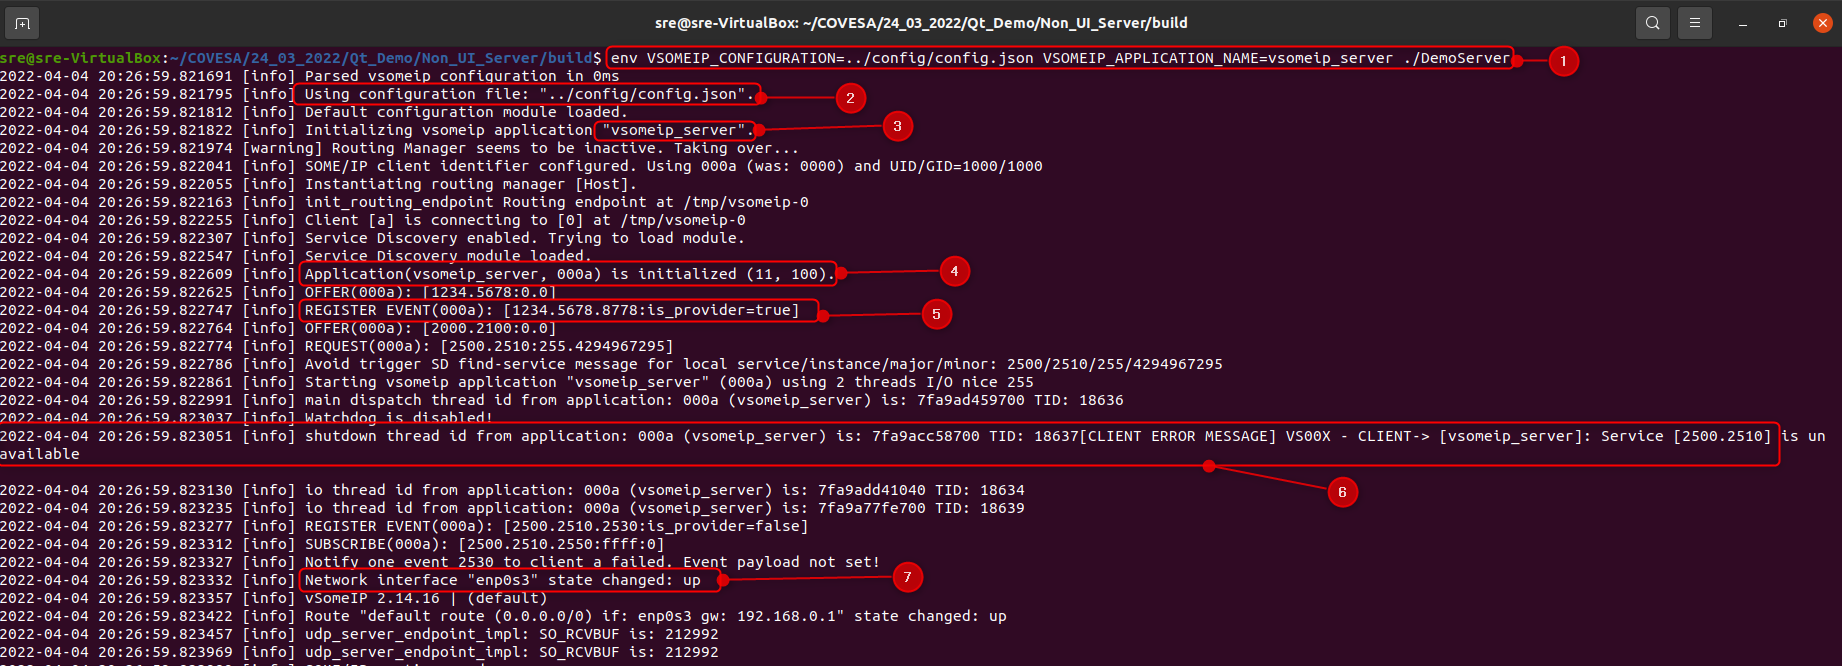
\includegraphics[width=1\textwidth]{images/res_server_eth0.png}
	\caption{Inter-ECU SOME/IP communication demonstration - Server}
	\label{fig:res_server_eth0}
\end{figure}


\subsection{Client Application Output}
\begin{figure}[!htb]
	\centering
		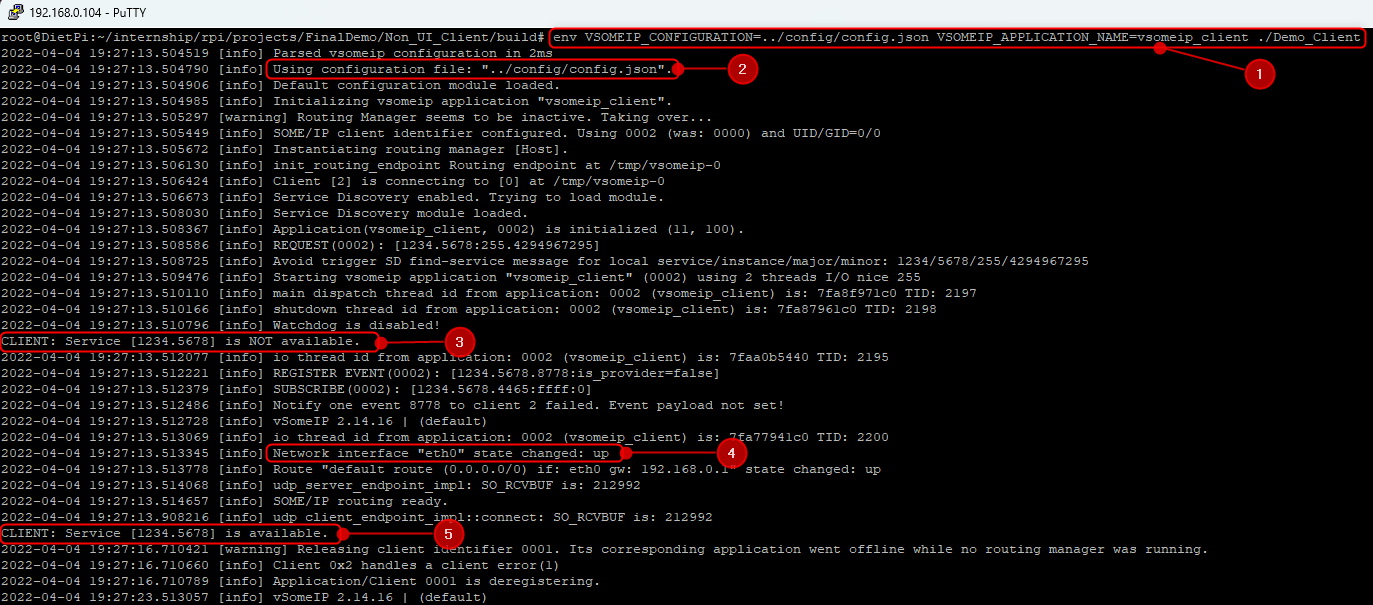
\includegraphics[width=1\textwidth]{images/res_client_eth0.png}
	\caption{Example of Inter-ECU SOME/IP communication - Client}
	\label{fig:res_client_eth0}
\end{figure}


\subsection{Troubleshooting guide}

\chapter{Conclusion}
Conclusion

%\chapter{Tables}
%% Example of, how to use a Table

\blindtext[1]

\begin{center}
\begin{tabular}{|c|c|c|c|}
\hline
Wert 1 & Wert 2 & Wert 3 & Wert 4\\
in Einheit1 & in Einheit2 & in Einheit3 & in Einheit4 \\
\hline
192 & 80& 0.3153 & 0.4900\\
500 & 120& 0.1229& 0.1787\\
1000 & 120& 0.0680& 0.0880\\
2000 & 120& 0.0361& 0.0441\\
5000 & 140& 0.0256& 0.0305\\
5000 & 164& 0.0343& 0.0880\\
\hline
\end{tabular}
\captionof{table}{This is the caption of the table}
\label{tab:table1}
\end{center}

\blindtext[3] % Load Data from File example_tables

%\chapter{Figures}
%% Example of, how to use figures

\blindtext

\begin{figure}[h]
\centering

\includegraphics[width=0.6\textwidth]{TU_Chemnitz_positiv_gruen.pdf}
\caption{Graphic 1}
\label{fig:pic0}
\end{figure}

\blindtext
\blindtext

\begin{figure}[h]
    \subfigure[This is the first graphic]{
\includegraphics[width=0.49\textwidth]{TU_Chemnitz_positiv_gruen.pdf} \label{fig:pic1}}
    \subfigure[This is the secound graphic]{
\includegraphics[width=0.49\textwidth]{TU_Chemnitz_positiv_gruen.pdf}\label{fig:pic2}}
\caption{This is the caption of the whole graphic}
\end{figure}

\blindtext

 % Load Data from File example_figures

%\chapter{Referencing}
% Alternativ just write your text under \chapter like this example

%\blindtext \cite{autorenrichtlinien}

%\blindtext \footnote{Here is an area for your Notes}

%\blindtext \footnote{\cite{lnilatex} Seite 11}
%\blindtext \cite{lnilatex}
%\blindtext \cite{autorenrichtlinien,pepper1992grundlagen,chen2001audiovisual}


%\chapter{Subchapter}

%\section{sub 1}
%\blindtext[3]
%\section{sub 2}
%\blindtext[3]
%\subsection{sub 2.1}
%\blindtext[3]

%\subsection{sub 2.2}
%\blindtext[3]

%---------------------------------------------------------
% bibliography based on Springer Design
%---------------------------------------------------------

%\bibliographystyle{splncs03}
%\bibliography{bibliography}

\def\BibTeX{{\rm B\kern-.05em{\sc i\kern-.025em b}\kern-.08em
    T\kern-.1667em\lower.7ex\hbox{E}\kern-.125emX}}
\printindex

\begin{thebibliography}{00}
\bibitem{b1}Kozierok, C. M., Correa, C., Boatright, R. B., \& Quesnelle, J. (2014). Automotive Ethernet: The Definitive Guide. Intrepid Control Systems.

\bibitem{b1.0}Zhang, H., Pan, Y., Lu, Z., Wang, J., \& Liu, Z. (2021). A Cyber Security Evaluation Framework for In-Vehicle Electrical Control Units. IEEE Access, 9, 149690-149706.

\bibitem{b1.0.1_AE_History}Hank, P., Müller, S., Vermesan, O., \& Van Den Keybus, J. (2013, March). Automotive ethernet: in-vehicle networking and smart mobility. In 2013 Design, Automation \& Test in Europe Conference \& Exhibition (DATE) (pp. 1735-1739). IEEE.

\bibitem{b1.0_EthBackbone}Han, S., \& Kim, H. (2016). On AUTOSAR TCP/IP performance in in-vehicle network environments. IEEE Communications Magazine, 54(12), 168-173.

\bibitem{b1.1}A. Ioana and A. Korodi, "VSOMEIP - OPC UA Gateway Solution for the Automotive Industry," 2019 IEEE International Conference on Engineering, Technology and Innovation (ICE/ITMC), 2019, pp. 1-6, doi: 10.1109/ICE.2019.8792619.

\bibitem{b1.2}G. L. Gopu, K. V. Kavitha and J. Joy, "Service Oriented Architecture based connectivity of automotive ECUs," 2016 International Conference on Circuit, Power and Computing Technologies (ICCPCT), 2016, pp. 1-4, doi: 10.1109/ICCPCT.2016.7530358.

\bibitem{b_middleware}Park, J., Kim, S., Yoo, W., \& Hong, S. (2006, October). Designing real-time and fault-tolerant middleware for automotive software. In 2006 SICE-ICASE International Joint Conference (pp. 4409-4413). IEEE.

\bibitem{b_TrendsInACS}Navet, N., Song, Y., Simonot-Lion, F., \& Wilwert, C. (2005). Trends in automotive communication systems. Proceedings of the IEEE, 93(6), 1204-1223.

\bibitem{b_someip_spec}“Some/IP protocol specification - AUTOSAR.” [Online]. Available: \url{https://www.autosar.org/fileadmin/user\_upload/standards/foundation/1-0/AUTOSAR\_PRS\_SOMEIPProtocol.pdf}. [Accessed: 11-Oct-2021]. 

\bibitem{b1.3}“Example for a Serialization Protocol (SOME/IP),” AUTOSAR Release 4.3.1, 31-Mar-2014. [Online]. Available: \url{https://www.autosar.org/fileadmin/user\_upload/standards/classic/4-1/AUTOSAR\_TR\_SomeIpExample.pdf}. [Accessed: 06-Nov-2022]. 

\bibitem{b1.4}Rumez, M., Grimm, D., Kriesten, R., \& Sax, E. (2020). An overview of automotive service-oriented architectures and implications for security countermeasures. IEEE access, 8, 221852-221870.

\bibitem{b_genivi_vsomeip}COVESA, “Covesa/vsomeip at 2.14.16,” GitHub. [Online]. Available: \url{https://github.com/COVESA/vsomeip/tree/2.14.16}. [Accessed: 14-Mar-2022]. 

\bibitem{scapy_someip}Jamores, “Jamores/ETH-Scapy-someip: Automotive ethernet some/IP-SD scapy protocol,” GitHub. [Online]. Available: \url{https://github.com/jamores/eth-scapy-someip}. [Accessed: 12-Nov-2021]. 

\bibitem{rust_someip}de Almeida, J. F. B. (2020). Rust-based SOME/IP implementation for robust automotive software.

\bibitem{b_adaptive_platform}AUTOSAR development cooperation, “Adaptive platform,” AUTOSAR, 06-Dec-2021. [Online]. Available: \url{https://www.autosar.org/standards/adaptive-platform/}. [Accessed: 18-Dec-2021]. 

\bibitem{b_commonapi}Covesa, “Releases · COVESA/CAPICXX-core-tools,” GitHub. [Online]. Available: \url{https://github.com/COVESA/capicxx-core-tools/releases?after=3.1.10.1}. [Accessed: 06-Jan-2021].

\bibitem{b_boost}Boost C++ libraries. [Online]. Available: \url{https://www.boost.org/users/history/version_1_65_0.html}. [Accessed: 10-Jan-2022].  

\bibitem{b_hyperv}Scooley, “Introduction to hyper-V on Windows 10,” Microsoft Docs. [Online]. Available: \url{https://docs.microsoft.com/en-us/virtualization/hyper-v-on-windows/about/}. [Accessed: 12-Nov-2021]. 

\bibitem{b_raspi3b}“Raspberry Pi 3 Model B+.,”  [Online]. Available: \url{https://datasheets.raspberrypi.com/rpi3/raspberry-pi-3-b-plus-product-brief.pdf}. [Accessed: 04-Nov-2021]. 

\bibitem{b_odroidxu4}“Odroid XU4 user Manual - Odroid Magazine.” [Online]. Available: \url{https://magazine.odroid.com/wp-content/uploads/odroid-xu4-user-manual.pdf}. [Accessed: 08-Nov-2021]. 

\bibitem{b_QtCreator}“Embedded Software Development Tools: Cross platform IDE: Qt creator,” Embedded Software Development Tools | Cross Platform IDE | Qt Creator. [Online]. Available: \url{https://www.qt.io/product/development-tools}. [Accessed: 06-Dec-2021]. 

\bibitem{b_CMake}“CMake Reference Documentation,” CMake Reference Documentation - CMake 3.23.0 Documentation. [Online]. Available: \url{https://cmake.org/cmake/help/latest/}. [Accessed: 12-Dec-2021]. 

\bibitem{b_putty}“Download Putty - a free SSH and telnet client for windows,” Download PuTTY - a free SSH and telnet client for Windows. [Online]. Available: https:\url{//www.putty.org/}. [Accessed: 17-Mar-2022]. 

\bibitem{b_vsomeip_userguide}Covesa. (2020, February 12). Vsomeip/vsomeipuserguide at master · COVESA/vsomeip. GitHub. Retrieved February 2, 2022, from \url{https://github.com/COVESA/vsomeip/blob/master/documentation/vsomeipUserGuide} 

\end{thebibliography}
\end{document}
